\documentclass[aspectratio=169,11pt]{beamer}

\usetheme{Madrid}
\usecolortheme{default}
\setbeamertemplate{navigation symbols}{}
\setbeamertemplate{footline}{%
  \leavevmode%
  \hbox{%
    \begin{beamercolorbox}[wd=.78\paperwidth,ht=2.5ex,dp=1.2ex,leftskip=1em]{author in head/foot}%
      \ifx\insertsection\empty Overview\else\insertsection\fi
    \end{beamercolorbox}%
    \begin{beamercolorbox}[wd=.22\paperwidth,ht=2.5ex,dp=1.2ex,center]{date in head/foot}%
      \insertframenumber{} / \inserttotalframenumber
    \end{beamercolorbox}%
  }%
}

\usepackage[T1]{fontenc}
\usepackage[utf8]{inputenc}
\usepackage{lmodern}
\usepackage{graphicx}
\usepackage{booktabs}
\usepackage{tabularx}
\usepackage{xcolor}
\usepackage{tikz}
\usetikzlibrary{arrows.meta,positioning}

\definecolor{accent}{RGB}{37,96,151}
\setbeamercolor{structure}{fg=accent}
\setbeamercolor{title}{fg=white,bg=accent}
\setbeamercolor{frametitle}{fg=white,bg=accent}

\newcommand{\code}[1]{\texttt{#1}}
\newcommand{\sectiontitle}[2]{%
\begin{frame}
\vfill
\centering
{\usebeamerfont{title}\color{accent}#1\par}
\vspace{0.5cm}
{\large #2\par}
\vfill
\end{frame}
}
\newcommand{\plot}[2]{%
\begin{center}
\includegraphics[width=\textwidth,height=0.78\textheight,keepaspectratio]{#1/#2}
\end{center}
}
\newcommand{\typelegend}{%
{\tiny\centering
\begin{tabular}{@{}llll@{}}
\textbf{A}: questions & \textbf{B}: boxes & \textbf{C}: captions & \textbf{E}: edit reconstruction \\
\textbf{G}: generation reconstruction & \textbf{L}: labels & \textbf{P}: preference & \textbf{R}: rating
\end{tabular}\par}
}
\newcommand{\typelegendab}{%
{\scriptsize\centering
\textbf{Types:} A = answering questions;\quad B = bounding boxes.\par}
}
\newcommand{\typeplot}[3]{%
\begin{center}
\includegraphics[width=\textwidth,height=#3,keepaspectratio]{#1/#2}
\end{center}
\vspace{-0.08cm}
\typelegend
}
\newcommand{\typeplotab}[3]{%
\begin{center}
\includegraphics[width=\textwidth,height=#3,keepaspectratio]{#1/#2}
\end{center}
\vspace{-0.08cm}
\typelegendab
}
\newcommand{\oldpair}{../../comparison/output/pre_jun11_gpt4o_vs_sonnet}
\newcommand{\oldpairab}{../../comparison/output/pre_jun11_gpt4o_vs_sonnet_type_ab}
\newcommand{\oldfive}{../../comparison/output/pre_jun11_five_api_models_old}
\newcommand{\studyfive}{../../comparison/output/five_api_models}
\newcommand{\newfive}{../../comparison/output/five_api_models_final_clean}
\newcommand{\finetune}{../../comparison/output/qwen25vl_finetuning}
\newcommand{\assetpath}{assets}
\newcommand{\benchasset}{../tex/images_benchmark_types}
\newcommand{\datasetasset}{../tex/images_datasets}
\newcommand{\uiasset}{../ui}
\newcommand{\datasetthumb}[3]{%
\begin{minipage}[t]{0.31\textwidth}
\centering
\includegraphics[width=\linewidth,height=0.18\textheight,keepaspectratio]{\datasetasset/#2}
\end{minipage}}

\title[Defense Results]{Defense Results Overview}
\subtitle{Historical API runs, five-model API comparison, and fine-tuning case study}
\author{}
\date{}

\begin{document}

\begin{frame}
\titlepage
\end{frame}

\section{Motivation}
\sectiontitle{Motivation}{Why a systematic VLM benchmark is needed}

\begin{frame}{Transformer and VLM Timeline}
\small
\begin{center}
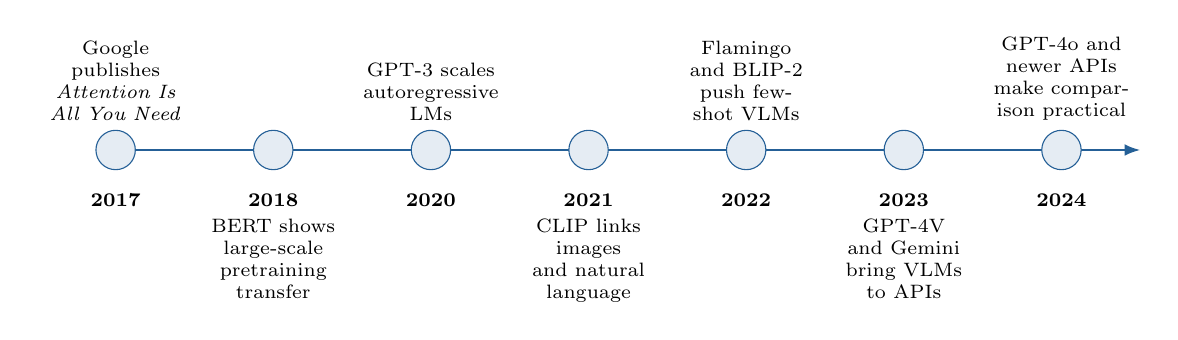
\begin{tikzpicture}[
    x=1.43cm,
    event/.style={circle,draw=accent,fill=accent!12,minimum size=0.5cm,inner sep=0pt},
    label/.style={align=center,text width=2.0cm,font=\scriptsize},
    >={Latex[length=2mm]}
]
\draw[->,thick,accent] (0,0) -- (9.1,0);
\node[event] (e2017) at (0,0) {};
\node[event] (e2018) at (1.4,0) {};
\node[event] (e2020) at (2.8,0) {};
\node[event] (e2021) at (4.2,0) {};
\node[event] (e2022) at (5.6,0) {};
\node[event] (e2023) at (7.0,0) {};
\node[event] (e2024) at (8.4,0) {};
\node[below=0.18cm of e2017,font=\scriptsize\bfseries] {2017};
\node[below=0.18cm of e2018,font=\scriptsize\bfseries] {2018};
\node[below=0.18cm of e2020,font=\scriptsize\bfseries] {2020};
\node[below=0.18cm of e2021,font=\scriptsize\bfseries] {2021};
\node[below=0.18cm of e2022,font=\scriptsize\bfseries] {2022};
\node[below=0.18cm of e2023,font=\scriptsize\bfseries] {2023};
\node[below=0.18cm of e2024,font=\scriptsize\bfseries] {2024};
\node[label,above=0.25cm] at (0,0) {Google publishes\\\textit{Attention Is All You Need}};
\node[label,below=0.75cm] at (1.4,0) {BERT shows large-scale\\pretraining transfer};
\node[label,above=0.25cm] at (2.8,0) {GPT-3 scales\\autoregressive LMs};
\node[label,below=0.75cm] at (4.2,0) {CLIP links images\\and natural language};
\node[label,above=0.25cm] at (5.6,0) {Flamingo and BLIP-2\\push few-shot VLMs};
\node[label,below=0.75cm] at (7.0,0) {GPT-4V and Gemini\\bring VLMs to APIs};
\node[label,above=0.25cm] at (8.4,0) {GPT-4o and newer APIs\\make comparison practical};
\end{tikzpicture}
\end{center}

\vspace{0.15cm}
\scriptsize
Transformer models moved from sequence modeling to general-purpose multimodal systems. This makes evaluation harder: model behavior depends on datasets, prompts, output parsing, metrics, provider APIs, and practical execution failures.
\end{frame}

\begin{frame}{Motivations}
\begin{center}
\Large
\begin{itemize}
    \item Measure models
    \item Measure datasets
\end{itemize}
\end{center}
\end{frame}

\section{Objectives}
\sectiontitle{Objectives}{Benchmark infrastructure instead of only a leaderboard}

\begin{frame}{Objectives: Main Aim}
\begin{itemize}
    \item Make comparisons systematic, reproducible, and extensible.
\end{itemize}
\end{frame}

\begin{frame}{Objectives: Concrete Goals}
\small
\begin{enumerate}
    \item Select a broad set of multimodal visual datasets with labels, captions, boxes, question-answer pairs, prompts, ratings, and preferences.
    \item Standardize dataset records through adapters that convert native formats into a common benchmark structure.
    \item Build benchmark tasks from dataset annotations: prompts, parsers, metrics, and task definitions.
    \item Integrate several vision-language models behind a shared image-plus-prompt interface.
    \item Compare model behavior across predictive performance, errors, runtime, coverage, and uncertainty.
    \item Keep the project extensible: adding a dataset mainly means adding an adapter; adding a model mainly means implementing the shared model interface.
\end{enumerate}
\end{frame}

\section{Dataset Selection}
\sectiontitle{Dataset Selection}{From literature search to standardized adapters}

\begin{frame}{Dataset Selection Procedure}
\scriptsize
\begin{center}
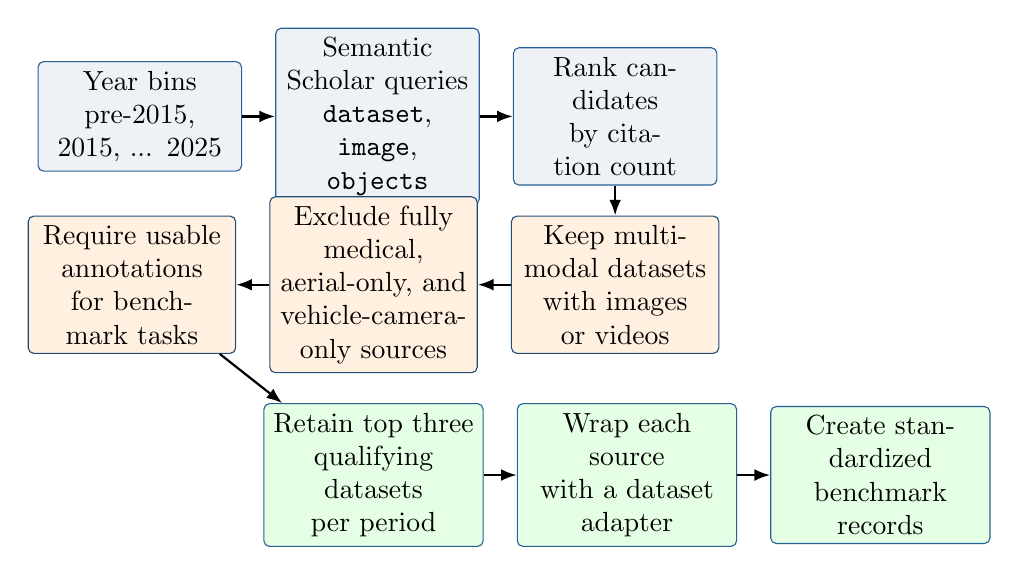
\begin{tikzpicture}[
    node distance=0.38cm and 0.42cm,
    box/.style={draw=accent,rounded corners=2pt,align=center,text width=2.35cm,minimum height=1.0cm,fill=accent!8},
    filter/.style={draw=accent!80!black,rounded corners=2pt,align=center,text width=2.4cm,minimum height=1.0cm,fill=orange!12},
    outputbox/.style={draw=accent,rounded corners=2pt,align=center,text width=2.55cm,minimum height=1.0cm,fill=green!10},
    >={Latex[length=2mm]}
]
\node[box] (periods) {Year bins\\pre-2015, 2015, ... 2025};
\node[box,right=of periods] (query) {Semantic Scholar queries\\\code{dataset}, \code{image}, \code{objects}};
\node[box,right=of query] (rank) {Rank candidates\\by citation count};
\node[filter,below=of rank] (vision) {Keep multimodal datasets\\with images or videos};
\node[filter,left=of vision] (scope) {Exclude fully medical, aerial-only, and vehicle-camera-only sources};
\node[filter,left=of scope] (available) {Require usable annotations\\for benchmark tasks};
\node[outputbox,below=of scope] (top) {Retain top three\\qualifying datasets per period};
\node[outputbox,right=of top] (adapter) {Wrap each source\\with a dataset adapter};
\node[outputbox,right=of adapter] (bench) {Create standardized\\benchmark records};

\draw[->,thick] (periods) -- (query);
\draw[->,thick] (query) -- (rank);
\draw[->,thick] (rank) -- (vision);
\draw[->,thick] (vision) -- (scope);
\draw[->,thick] (scope) -- (available);
\draw[->,thick] (available) -- (top);
\draw[->,thick] (top) -- (adapter);
\draw[->,thick] (adapter) -- (bench);
\end{tikzpicture}
\end{center}

\vspace{0.08cm}
\scriptsize
The selection favors historically visible multimodal datasets while filtering for sources that can be converted into repeatable visual benchmark tasks.
\end{frame}

\begin{frame}{Selected Datasets by Publication Year}
\tiny
\begin{columns}[T,totalwidth=\textwidth]
\begin{column}{0.32\textwidth}
\textbf{Pre-2015}\\
ImageNet (2009); UCF101 (2012); MS COCO (2014)

\textbf{2015}\\
Flickr30k Entities; FlyingThings3D; LSUN

\textbf{2016}\\
Cityscapes; Visual Genome; VQA v2.0

\textbf{2017}\\
Fashion-MNIST; Kinetics Human Action Video Dataset; iNaturalist
\end{column}
\begin{column}{0.32\textwidth}
\textbf{2018}\\
Places; Conceptual Captions; Open Images V4

\textbf{2019}\\
GQA; MVTec AD; LVIS

\textbf{2020}\\
DocVQA; DFDC; TextCaps

\textbf{2021}\\
LAION-400M; FairFace; HDTF
\end{column}
\begin{column}{0.32\textwidth}
\textbf{2022}\\
LAION-5B; DiffusionDB; TAD66K

\textbf{2023}\\
MagicBrush; Pick-a-Pic; InternVid

\textbf{2024}\\
OpenVid-1M; Visual CoT; HQ-Edit

\textbf{2025}\\
BLIP3o-60k; ImgEdit; ShareGPT-4o-Image
\end{column}
\end{columns}
\end{frame}

\begin{frame}{Dataset Example: ImageNet}
\begin{center}

\includegraphics[width=\textwidth,height=0.72\textheight,keepaspectratio]{\datasetasset/ImageNet.JPG}
\end{center}
\end{frame}

\begin{frame}{Dataset Example: MS COCO}
\begin{center}

\includegraphics[width=\textwidth,height=0.72\textheight,keepaspectratio]{\datasetasset/MSCOCO.JPG}
\end{center}
\end{frame}

\begin{frame}{Dataset Example: DocVQA}
\begin{center}

\includegraphics[width=\textwidth,height=0.72\textheight,keepaspectratio]{\datasetasset/DocVQA.JPG}
\end{center}
\end{frame}

\begin{frame}{Dataset Example: MagicBrush}
\begin{center}

\includegraphics[width=\textwidth,height=0.72\textheight,keepaspectratio]{\datasetasset/MagicBrush.JPG}
\end{center}
\end{frame}

\section{Model Selection}
\sectiontitle{Model Selection}{Comparable API models through one interface}

\begin{frame}{Model Selection}
\scriptsize
\begin{tabularx}{\textwidth}{@{}p{2.6cm}p{3.0cm}X@{}}
\toprule
\textbf{Model family} & \textbf{API model ID} & \textbf{Reason for inclusion} \\
\midrule
OpenAI flagship VLM & \code{gpt-4o} & Strong widely used multimodal baseline available during the first API run. \\
OpenAI later model & \code{gpt-4.1} & Included to compare a newer OpenAI API model against GPT-4o and GPT-5. \\
OpenAI reasoning-era model & \code{gpt-5} & Evaluated as exactly \code{gpt-5} with \code{reasoning.effort=minimal}; not a GPT-5.1 or GPT-5.2 run. \\
Anthropic Claude & \code{claude-sonnet-4-5} & Independent provider baseline with strong vision-language performance. \\
Google Gemini & \code{gemini-3.5-flash} & Fast Google VLM API model; configured with \code{thinking\_budget=0} when supported. \\
\bottomrule
\end{tabularx}

\vspace{0.2cm}
\scriptsize
All models are called through the same benchmark-facing interface: image plus prompt in, text response out, then shared parsing and scoring.
\end{frame}

\section{Overview}
\begin{frame}{Four Result Sets}
\begin{enumerate}
    \item June 10 GPT-4o vs. Claude Sonnet comparison.
    \item Five-model study comparison on 21 shared benchmarks.
    \item Five-model full comparison on 44 benchmarks.
    \item Qwen2.5-VL-3B Fashion-MNIST fine-tuning case study.
\end{enumerate}
\end{frame}

\section{Benchmark types}
\sectiontitle{Benchmark types}{One example for each evaluated task family}

\begin{frame}{Type A: Answering Questions}
\begin{center}

\includegraphics[width=0.92\textwidth,height=0.48\textheight,keepaspectratio]{\benchasset/type_a_flyingthings3d_03.png}
\end{center}
\vspace{-0.08cm}
\scriptsize
\textbf{Benchmark:} \code{flyingthings3d}, example 3

\vspace{0.06cm}
\textbf{Prompt:} What part of the gray car is most visible?

\textbf{Choices:} A. the front; B. the back; C. the side; D. the top.

\vspace{0.06cm}
\textbf{Reference:} the back

\textbf{GPT-4o response:} C. the side

\textbf{Score:} accuracy \(=0\) (incorrect)
\end{frame}

\begin{frame}{Type B: Bounding Box Detection}
\begin{columns}[T,totalwidth=\textwidth]
\begin{column}{0.48\textwidth}

\includegraphics[width=\textwidth,height=0.64\textheight,keepaspectratio]{\benchasset/type_b_mscoco_02_correct_boxes.png}
\end{column}
\begin{column}{0.49\textwidth}
\scriptsize
\textbf{Benchmark:} \code{mscoco}, example 2

\vspace{0.08cm}
\textbf{Target class:} chair

\textcolor{red!80!black}{\textbf{GPT-4o response:}} \code{[0.0, 0.6, 0.3, 0.4]}

\textbf{Score:} F1 \(=0.000\), matched IoU \(=0.000\)

\vspace{0.08cm}
\textcolor{green!50!black}{\textbf{Correct boxes}} \([x,y,w,h]\), normalized:
\begin{itemize}
    \item \code{[0.08, 0.94, 0.17, 0.06]}
    \item \code{[0.33, 0.82, 0.14, 0.11]}
    \item \code{[0.69, 0.78, 0.15, 0.20]}
\end{itemize}
\end{column}
\end{columns}
\end{frame}

\begin{frame}{Type C: Captioning}
\begin{columns}[T,totalwidth=\textwidth]
\begin{column}{0.46\textwidth}

\includegraphics[width=\textwidth,height=0.66\textheight,keepaspectratio]{\benchasset/type_c_conceptual_captions_02.png}
\end{column}
\begin{column}{0.51\textwidth}
\scriptsize
\textbf{Benchmark:} \code{conceptual\_captions\_caption}, example 2

\vspace{0.12cm}
\textbf{Prompt:} Write one concise caption for the image.

\textbf{Reference:} the - bedroom stone cottage can sleep people

\textbf{GPT-4o response:} Cozy bedroom with wooden flooring and modern decor.

\textbf{Score:} BLEU \(=0.1604\) (incorrect)
\end{column}
\end{columns}
\end{frame}

\begin{frame}{Type E: Editing Reconstruction}
\begin{columns}[T,totalwidth=\textwidth]
\begin{column}{0.50\textwidth}

\includegraphics[width=\textwidth,height=0.66\textheight,keepaspectratio]{\benchasset/type_e_hq_edit_05.png}
\end{column}
\begin{column}{0.47\textwidth}
\scriptsize
\textbf{Benchmark:} \code{hq\_edit}, example 5

\vspace{0.12cm}
\textbf{Prompt:} Identify which edit instruction produced Image B from Image A.

\vspace{0.06cm}
\textbf{Options:}
\begin{enumerate}
    \item[A.] Replace the soccer ball with a miniature sunflower that the puppy is holding.
    \item[B.] Replace the soccer ball with a miniature sunflower that the kitten is holding.
    \item[C.] Replace the soccer ball with a giant sunflower that the puppy is holding.
    \item[D.] Replace the soccer ball with a giant sunflower that the kitten is holding.
\end{enumerate}

\textbf{Reference:} replace the soccer ball with a giant sunflower that the puppy is holding.

\textbf{GPT-4o response:} C. Replace the soccer ball with a giant sunflower that the puppy is holding.

\textbf{Score:} accuracy \(=1\) (correct)
\end{column}
\end{columns}
\end{frame}

\begin{frame}{Type G: Generating Reconstruction}
\begin{columns}[T,totalwidth=\textwidth]
\begin{column}{0.46\textwidth}

\includegraphics[width=\textwidth,height=0.66\textheight,keepaspectratio]{\benchasset/type_g_diffusiondb_02.png}
\end{column}
\begin{column}{0.51\textwidth}
\scriptsize
\textbf{Benchmark:} \code{diffusiondb}, example 2

\vspace{0.12cm}
\textbf{Prompt:} Identify which prompt created the image from four choices.

\vspace{0.06cm}
\textbf{Options:}
\begin{enumerate}
    \item[A.] renaissance portrait of Dwayne Johnson, Rembrandt style\ldots
    \item[B.] epic 3D GPU mecha controlled by telepathic hackers\ldots
    \item[C.] airbrush painting of cyber war machine scene in Area 51\ldots
    \item[D.] portrait of a dancing eagle woman, Lakota Sioux goddess\ldots
\end{enumerate}

\textbf{Reference:} choice D, a portrait of a dancing eagle woman.

\textbf{GPT-4o response:} D

\textbf{Score:} accuracy \(=1\) (correct)
\end{column}
\end{columns}
\end{frame}

\begin{frame}{Type L: Labeling}
\begin{columns}[T,totalwidth=\textwidth]
\begin{column}{0.46\textwidth}

\includegraphics[width=\textwidth,height=0.66\textheight,keepaspectratio]{\benchasset/type_l_imagenet1k_01.png}
\end{column}
\begin{column}{0.51\textwidth}
\scriptsize
\textbf{Benchmark:} \code{imagenet1k}, example 1

\vspace{0.12cm}
\textbf{Prompt:} Return exactly one label from the ImageNet-1K label list.

\vspace{0.06cm}
\textbf{Label list head sent to model:}
\begin{enumerate}
    \item tench, Tinca tinca
    \item goldfish, Carassius auratus
    \item great white shark, white shark, man-eater\ldots
    \item tiger shark, Galeocerdo cuvieri
    \item hammerhead, hammerhead shark
    \item electric ray, crampfish, numbfish, torpedo
\end{enumerate}

\textbf{Reference:} sombrero

\textbf{GPT-4o response:} sombrero

\textbf{Score:} accuracy \(=1\) (correct)
\end{column}
\end{columns}
\end{frame}

\begin{frame}{Type P: Preference}
\begin{columns}[T,totalwidth=\textwidth]
\begin{column}{0.54\textwidth}

\includegraphics[width=\textwidth,height=0.64\textheight,keepaspectratio]{\benchasset/type_p_pick_a_pic_04.png}
\end{column}
\begin{column}{0.43\textwidth}
\scriptsize
\textbf{Benchmark:} \code{pick\_a\_pic}, example 4

\vspace{0.12cm}
\textbf{Prompt:} Which image is more aesthetically pleasing overall?

\textbf{Reference:} Image A

\textbf{GPT-4o response:} A

\textbf{Score:} accuracy \(=1\) (correct)
\end{column}
\end{columns}
\end{frame}

\begin{frame}{Type R: Rating}
\begin{columns}[T,totalwidth=\textwidth]
\begin{column}{0.46\textwidth}

\includegraphics[width=\textwidth,height=0.66\textheight,keepaspectratio]{\benchasset/type_r_tad66k_06.png}
\end{column}
\begin{column}{0.51\textwidth}
\scriptsize
\textbf{Benchmark:} \code{tad66k}, example 6

\vspace{0.12cm}
\textbf{Prompt:} Rate the overall aesthetic quality from 1 to 10.

\textbf{Reference:} 7

\textbf{GPT-4o response:} 7

\textbf{Score:} absolute error \(=0\) (correct)
\end{column}
\end{columns}
\end{frame}

\begin{frame}{Dataset UI}
\begin{center}

\includegraphics[width=\textwidth,height=0.80\textheight,keepaspectratio]{\uiasset/dataset_ui_0.PNG}
\end{center}
\end{frame}

\begin{frame}{Dataset UI}
\begin{center}

\includegraphics[width=\textwidth,height=0.80\textheight,keepaspectratio]{\uiasset/dataset_ui_1.PNG}
\end{center}
\end{frame}

\begin{frame}{Dataset UI}
\begin{center}

\includegraphics[width=\textwidth,height=0.80\textheight,keepaspectratio]{\uiasset/dataset_ui_2.PNG}
\end{center}
\end{frame}

\begin{frame}{Dataset UI}
\begin{center}

\includegraphics[width=\textwidth,height=0.80\textheight,keepaspectratio]{\uiasset/dataset_ui_3.PNG}
\end{center}
\end{frame}

\section{June 10 GPT-4o vs. Sonnet}
\sectiontitle{Results 1}{June 10 GPT-4o vs. Claude Sonnet}

\begin{frame}{Evaluated API Models}
\tiny
\begin{tabularx}{\textwidth}{@{}p{2.8cm}p{2.8cm}X@{}}
\toprule
\textbf{Slide label} & \textbf{API model ID} & \textbf{What was actually requested} \\
\midrule
\code{gpt-4o} & \code{gpt-4o} &
OpenAI Responses API vision request; deterministic setting with \code{temperature=0.0}. \\
\code{gpt-4.1} & \code{gpt-4.1} &
OpenAI Responses API vision request; deterministic setting with \code{temperature=0.0}. \\
\code{gpt-5} & \code{gpt-5} &
OpenAI Responses API vision request with \code{reasoning.effort=minimal}; not \code{gpt-5.1}, \code{gpt-5.2}, or a ChatGPT UI mode label. \\
\code{claude-sonnet-4-5} & \code{claude-sonnet-4-5} &
Anthropic Messages API vision request; \code{temperature=0.0}. \\
\code{gemini-3.5-flash} & \code{gemini-3.5-flash} &
Google GenAI vision request; \code{temperature=0.0} and \code{thinking\_budget=0} when supported by the SDK. \\
\bottomrule
\end{tabularx}

\vspace{0.2cm}
{\scriptsize The June 10 comparison uses only \code{gpt-4o} and \code{claude-sonnet-4-5};
the later five-model comparisons use all rows above.}
\end{frame}

\begin{frame}{Results 1: Overall Summary}
\begin{minipage}[t]{0.45\textwidth}
\scriptsize
\resizebox{\textwidth}{!}{%
\begin{tabularx}{\textwidth}{@{}lrr@{}}
\toprule
\textbf{Model} & \textbf{Mean} & \textbf{Median} \\
\midrule
\code{gpt-4o} & 0.428 & 0.327 \\
\code{claude-sonnet-4-5} & 0.368 & 0.225 \\
\bottomrule
\end{tabularx}
}

\vspace{0.25cm}
\begin{itemize}
    \item GPT-4o wins 19 benchmarks, Sonnet wins 8, and 3 are tied.
    \item Mean score delta is +0.061 for GPT-4o.
\end{itemize}
\end{minipage}\hfill
\begin{minipage}[t]{0.45\textwidth}

\includegraphics[width=\textwidth,height=0.63\textheight,keepaspectratio]{\assetpath/results1_model_mean_scores_tall.png}
\end{minipage}
\end{frame}

\begin{frame}{Results 1: Benchmark Heatmap}
\small
\textbf{Pearson correlation:} \(\mathbf{r=0.891}\)

\vspace{0.06cm}
\begin{center}

\includegraphics[width=\textwidth,height=0.78\textheight,keepaspectratio]{\assetpath/results1_score_heatmap_raw_flipped.png}
\end{center}
\end{frame}

\begin{frame}{Results 1: Benchmark Types}
\typeplot{\oldpair}{family_grouped_bars.png}{0.66\textheight}
\end{frame}

\begin{frame}{Actual Sample Type B: iNaturalist Detection}
\begin{columns}[T,totalwidth=\textwidth]
\begin{column}{0.52\textwidth}

\includegraphics[width=\textwidth,height=0.66\textheight,keepaspectratio]{\assetpath/type_b_examples/inaturalist_detection_sample_09.png}
\vspace{0.05cm}

{\scriptsize Target: \emph{Jabiru mycteria}. Green: correct box. Blue: GPT-4o. Red: Sonnet.}
\end{column}
\begin{column}{0.45\textwidth}
\scriptsize
\textbf{Prompt:} Detect all visible instances of \emph{Jabiru mycteria}. Return normalized \([x,y,w,h]\) boxes only, or [] if none.

\vspace{0.15cm}
\textbf{GPT-4o answer:} {\ttfamily [0.2, 0.3, 0.2, 0.4]}\\
\textbf{GPT-4o score:} F1=0.00, P=0.00, R=0.00

\vspace{0.15cm}
\textbf{Sonnet answer:} {\ttfamily [0.0, 0.15, 0.55, 0.85]}\\
\textbf{Sonnet score:} F1=1.00, P=1.00, R=1.00
\end{column}
\end{columns}
\end{frame}

\begin{frame}{Actual Sample Type C: Flickr30K Captioning}
\begin{columns}[T,totalwidth=\textwidth]
\begin{column}{0.52\textwidth}

\includegraphics[width=\textwidth,height=0.72\textheight,keepaspectratio]{\assetpath/type_c_flickr30k_sample2.png}
\end{column}
\begin{column}{0.45\textwidth}
\scriptsize
\textbf{Prompt:} Write one concise caption for the image.

\vspace{0.15cm}
\textbf{Reference captions include:}
\begin{itemize}
    \item Several men in hard hats are operating a giant pulley system.
    \item Four men on top of a tall structure.
\end{itemize}

\vspace{0.12cm}
\textbf{GPT-4o answer:} Workers performing maintenance on a tall construction crane.\\
\textbf{GPT-4o score:} correct

\vspace{0.12cm}
\textbf{Sonnet answer:} Workers on a crane lift a large hook or pulley system during construction or maintenance work.\\
\textbf{Sonnet score:} incorrect
\end{column}
\end{columns}
\end{frame}

\begin{frame}{Actual Sample Type L: Conceptual Captions}
\begin{columns}[T,totalwidth=\textwidth]
\begin{column}{0.52\textwidth}

\includegraphics[width=\textwidth,height=0.72\textheight,keepaspectratio]{\assetpath/type_l_examples/conceptual_captions_sample_18.png}
\end{column}
\begin{column}{0.45\textwidth}
\scriptsize
\textbf{Prompt:} Select the matching caption from four options.

\vspace{0.15cm}
\textbf{Correct answer:} keeping fans informed : since their birth in january this year, the couple have been keeping fans updated with the babies progress

\vspace{0.15cm}
\textbf{GPT-4o answer:} [no answer returned]\\
\textbf{GPT-4o score:} accuracy=0, error

\vspace{0.15cm}
\textbf{Sonnet answer:} B\\
\textbf{Sonnet score:} accuracy=1
\end{column}
\end{columns}
\end{frame}

\begin{frame}{Results 1: Type A/B Summary}
\small
\begin{tabularx}{\textwidth}{@{}llrrr@{}}
\toprule
\textbf{Type} & \textbf{Model} & \textbf{Benchmarks} & \textbf{Mean} & \textbf{Mean rank} \\
\midrule
Type A & \code{gpt-4o} & 6 & 0.800 & 1.00 \\
Type A & \code{claude-sonnet-4-5} & 6 & 0.508 & 2.00 \\
Type B & \code{gpt-4o} & 6 & 0.100 & 1.33 \\
Type B & \code{claude-sonnet-4-5} & 6 & 0.135 & 1.50 \\
\bottomrule
\end{tabularx}

\vspace{0.35cm}
GPT-4o is clearly ahead on Type A. Type B is more mixed: Sonnet has the
higher raw mean, while GPT-4o has the better average rank.
\end{frame}

\begin{frame}{Results 1: Type A/B Types}
\typeplotab{\oldpairab}{family_grouped_bars.png}{0.68\textheight}
\end{frame}

\section{21-Benchmark Study Comparison}
\sectiontitle{Results 2}{21-Benchmark Study Comparison}

\begin{frame}{21-Benchmark Study: Error Counts}
\small
\textbf{420 samples per model}

\vspace{0.22cm}
\begin{tabularx}{\textwidth}{@{}lrr@{}}
\toprule
\textbf{Model} & \textbf{Errors} & \textbf{Error rate} \\
\midrule
\code{claude-sonnet-4-5} & 15 & 3.6\% \\
\code{gemini-3.5-flash} & 236 & 56.2\% \\
\code{gpt-4.1} & 195 & 46.4\% \\
\code{gpt-4o} & 15 & 3.6\% \\
\code{gpt-5} & 199 & 47.4\% \\
\bottomrule
\end{tabularx}
\end{frame}

\begin{frame}{21-Benchmark Study: Old Type A/B/C Results}
\begin{center}

\includegraphics[width=\textwidth,height=0.78\textheight,keepaspectratio]{\assetpath/study21_type_abc_old.png}
\end{center}
\end{frame}

\begin{frame}{21-Benchmark Study: New Clean Type A/B/C Results}
\begin{center}

\includegraphics[width=\textwidth,height=0.78\textheight,keepaspectratio]{\assetpath/study21_type_abc_new_clean.png}
\end{center}
\end{frame}

\begin{frame}{21-Benchmark Study: Pairwise Wins}
\plot{\assetpath}{study21_final_pairwise_win_rate_heatmap.png}
\end{frame}

\begin{frame}{21-Benchmark Study: Clean Raw Score Heatmap}
\begin{center}

\includegraphics[width=\textwidth,height=0.78\textheight,keepaspectratio]{\assetpath/study21_clean_raw_heatmap.png}
\end{center}
\end{frame}

\begin{frame}{21-Benchmark Study: Bootstrap Intervals}
\begin{center}

\includegraphics[width=\textwidth,height=0.72\textheight,keepaspectratio]{\assetpath/study21_clean_bootstrap_intervals.png}
\end{center}
\vspace{-0.08cm}
{\scriptsize Horizontal intervals show the 5th--95th percentile range of bootstrapped mean raw scores over the 21 clean benchmarks.}
\end{frame}

\begin{frame}{21-Benchmark Study: Type A/B/C Radar}
\begin{center}

\includegraphics[width=\textwidth,height=0.78\textheight,keepaspectratio]{\assetpath/study21_clean_type_abc_radar.png}
\end{center}
\end{frame}

\begin{frame}{21-Benchmark Study: Model Similarity}
\begin{center}

\includegraphics[width=\textwidth,height=0.78\textheight,keepaspectratio]{\assetpath/study21_clean_model_similarity_heatmap.png}
\end{center}
\end{frame}

\begin{frame}{21-Benchmark Study: 2D Model Map}
\begin{center}

\includegraphics[width=\textwidth,height=0.78\textheight,keepaspectratio]{\assetpath/study21_clean_model_pca_map.png}
\end{center}
\end{frame}

\begin{frame}{21-Benchmark Study: Performance vs. Latency}
\begin{center}

\includegraphics[width=\textwidth,height=0.78\textheight,keepaspectratio]{\assetpath/study21_clean_perf_vs_latency.png}
\end{center}
\end{frame}

\begin{frame}{21-Benchmark Study: Difficulty vs. Separation}
\begin{center}

\includegraphics[width=\textwidth,height=0.78\textheight,keepaspectratio]{\assetpath/study21_clean_benchmark_difficulty_discrimination.png}
\end{center}
\end{frame}

\begin{frame}{21-Benchmark Study: Price vs. Average Score}
\begin{center}

\includegraphics[width=\textwidth,height=0.78\textheight,keepaspectratio]{\assetpath/study21_price_vs_average_score.png}
\end{center}
\end{frame}

\begin{frame}{21-Benchmark Study: Release Year vs. Average Score}
\begin{center}

\includegraphics[width=\textwidth,height=0.78\textheight,keepaspectratio]{\assetpath/study21_release_year_vs_average_score.png}
\end{center}
\end{frame}

\section{44-Benchmark Full Comparison}
\sectiontitle{Results 3}{44-Benchmark Full Comparison}

\begin{frame}{44-Benchmark Full: Setup}
\begin{itemize}
    \item Source: \code{results/api\_models\_final\_clean}.
    \item Balanced run: 44 benchmarks for each of five API models.
    \item Total: 220 benchmark files and 4,345 sample results.
    \item No sample-level errors.
\end{itemize}
\end{frame}

\begin{frame}{44-Benchmark Full: Summary}
\small
\begin{tabularx}{\textwidth}{@{}lrrrr@{}}
\toprule
\textbf{Model} & \textbf{Mean} & \textbf{Median} & \textbf{Normalized} & \textbf{Mean rank} \\
\midrule
\code{gemini-3.5-flash} & 0.585 & 0.725 & 0.790 & 1.82 \\
\code{gpt-4.1} & 0.559 & 0.625 & 0.668 & 2.18 \\
\code{gpt-5} & 0.519 & 0.625 & 0.567 & 2.66 \\
\code{gpt-4o} & 0.509 & 0.550 & 0.573 & 2.70 \\
\code{claude-sonnet-4-5} & 0.419 & 0.393 & 0.254 & 3.82 \\
\bottomrule
\end{tabularx}
\end{frame}

\begin{frame}{44-Benchmark Full: Benchmark Heatmap}
\small
\textbf{Mean pairwise Pearson correlation:} \(\mathbf{r=-0.014}\)

\vspace{0.06cm}
\begin{center}

\includegraphics[width=\textwidth,height=0.72\textheight,keepaspectratio]{\assetpath/results3_score_heatmap_normalized_flipped.png}
\end{center}
\end{frame}

\begin{frame}{44-Benchmark Full: Benchmark Type Leaders}
\typeplot{\newfive}{family_grouped_bars.png}{0.66\textheight}
\end{frame}

\begin{frame}{44-Benchmark Full: Model Correlations}
\begin{center}

\includegraphics[width=\textwidth,height=0.78\textheight,keepaspectratio]{\assetpath/full44_model_pairwise_correlation.png}
\end{center}
\end{frame}

\begin{frame}{44-Benchmark Full: Average vs. Standard Deviation}
\begin{center}

\includegraphics[width=\textwidth,height=0.78\textheight,keepaspectratio]{\assetpath/full44_average_score_vs_std.png}
\end{center}
\end{frame}

\section{Fine-Tuning Case Study}
\sectiontitle{Results 4}{Qwen2.5-VL-3B Fashion-MNIST Fine-Tuning}

\begin{frame}{Results 4: Setup}
\scriptsize
\begin{tabularx}{\textwidth}{@{}p{2.7cm}X@{}}
\toprule
\textbf{Component} & \textbf{Details} \\
\midrule
Base model & \code{Qwen/Qwen2.5-VL-3B-Instruct}. \\
Task and data & Fashion-MNIST classification; 100 train examples and 20 validation examples from the train split; 50 ordered test examples for evaluation. \\
Compared systems & Unmodified baseline; original Fashion-MNIST LoRA adapter; balanced Fashion-MNIST LoRA adapter. \\
Balanced variant & Uses a class-balanced Fashion-MNIST training/validation selection; same base model and evaluation set. \\
QLoRA setup & 4-bit NF4 quantization with double quantization; LoRA rank 16, alpha 32, dropout 0.05. \\
Trainable modules & Attention projections only: \code{q\_proj}, \code{k\_proj}, \code{v\_proj}, and \code{o\_proj}. \\
Training defaults & 2 epochs, learning rate \(10^{-4}\), batch size 1, gradient accumulation 8, warmup 5, seed 42; best checkpoint selected by validation loss. \\
\bottomrule
\end{tabularx}
\end{frame}

\begin{frame}{Results 4: Accuracy Summary}
\small
\begin{tabularx}{\textwidth}{@{}lrrrr@{}}
\toprule
\textbf{Model} & \textbf{Correct} & \textbf{Accuracy} & \textbf{Macro recall} & \textbf{Macro F1} \\
\midrule
Baseline & 19/50 & 0.380 & 0.368 & 0.342 \\
Original LoRA & 19/50 & 0.380 & 0.349 & 0.296 \\
Balanced LoRA & 24/50 & 0.480 & 0.455 & 0.455 \\
\bottomrule
\end{tabularx}

\vspace{0.35cm}
The balanced adapter gives a 10-point accuracy gain and a 16.1\% relative
error reduction.
\end{frame}

\begin{frame}{Results 4: Accuracy}
\plot{\finetune}{accuracy_comparison.png}
\end{frame}

\begin{frame}{Results 4: Confusion Matrices}
\begin{center}

\includegraphics[width=\textwidth,height=0.58\textheight,keepaspectratio]{\finetune/confusion_matrices.png}
\end{center}
\vspace{-0.08cm}
{\tiny
\textbf{Class index:}
0 T-shirt/top;\quad
1 trouser;\quad
2 pullover;\quad
3 dress;\quad
4 coat;\quad
5 sandal;\quad
6 shirt;\quad
7 sneaker;\quad
8 bag;\quad
9 ankle boot.
\par}
\end{frame}

\begin{frame}{Results 4: Prediction Distribution}
\plot{\finetune}{prediction_distribution.png}
\end{frame}

\begin{frame}{Results 4: Original LoRA Training Labels}
\small
\begin{columns}[T,totalwidth=\textwidth]
\begin{column}{0.46\textwidth}
\begin{tabular}{@{}lr@{}}
\toprule
\textbf{Class} & \textbf{Train examples} \\
\midrule
Ankle boot & 5 \\
Bag & 10 \\
Coat & 13 \\
Dress & 9 \\
Pullover & 9 \\
Sandal & 12 \\
\textbf{Shirt} & \textbf{16} \\
Sneaker & 13 \\
T-shirt/top & 10 \\
Trouser & 3 \\
\bottomrule
\end{tabular}
\end{column}
\begin{column}{0.50\textwidth}
\begin{itemize}
    \item Original LoRA used 100 Fashion-MNIST training examples.
    \item The class distribution was uneven.
    \item \textbf{Shirt} was the largest class with 16 examples.
    \item This helps explain why the original adapter over-predicts shirt in the confusion matrix.
\end{itemize}
\end{column}
\end{columns}
\end{frame}

\end{document}
